\documentclass[manuscript,review,anonymous]{acmart}

%% ------------------------------------------------------------------
%% BASiS: Bayesian Style-based Selection
%% IUI 2027 double-blind submission draft
%% Compile with pdflatex (or latexmk -pdf) + bibtex.
%% ------------------------------------------------------------------

\usepackage{amsmath}
\usepackage{booktabs}
\usepackage{graphicx}
\usepackage{tabularx}
\usepackage{array}
\usepackage{colortbl}
\usepackage{collcell}
\usepackage{comment}

%% Long-table layout switch.  Change only the following line to
%% \BasisPolishedTablesfalse to restore the previous centered layout with
%% underlined corpus-pair headings in Tables 3 and 4.
\newif\ifBasisPolishedTables
\BasisPolishedTablestrue
\definecolor{basisTableGroup}{gray}{0.95}
\newcommand{\BasisCorpusHeader}[1]{%
  \ifBasisPolishedTables
    \rowcolor{basisTableGroup}%
    \multicolumn{2}{c}{\strut\textbf{#1}} \\
  \else
    \multicolumn{2}{c}{\textbf{#1}} \\
    \cmidrule(lr){1-2}
  \fi
}
\newcommand{\BasisFinalChoiceLabel}[1]{%
  \ifBasisPolishedTables\mbox{\textbf{#1}}\else#1\fi
}
\ifBasisPolishedTables
  \newcommand{\BasisOracleTableWidth}{0.98\textwidth}
  \newcommand{\BasisOracleAxisWidth}{0.34\textwidth}
  \newcommand{\BasisHumanTableWidth}{0.98\textwidth}
  \newcolumntype{A}{>{\raggedleft\arraybackslash}p{\BasisOracleAxisWidth}}
  \newcolumntype{I}{>{\raggedleft\arraybackslash}p{0.11\textwidth}}
  \newcolumntype{Q}{>{\raggedright\arraybackslash}X}
\else
  \newcommand{\BasisOracleTableWidth}{0.98\textwidth}
  \newcommand{\BasisOracleAxisWidth}{0.30\textwidth}
  \newcommand{\BasisHumanTableWidth}{0.96\textwidth}
  \newcolumntype{A}{>{\centering\arraybackslash}p{\BasisOracleAxisWidth}}
  \newcolumntype{I}{>{\centering\arraybackslash}p{0.08\textwidth}}
  \newcolumntype{Q}{>{\centering\arraybackslash}X}
\fi

%% Uncomment once the submission ID has been issued by PCS.
%% \acmSubmissionID{123-A45-B67}

\setcopyright{acmlicensed}
\acmConference[IUI '27]{32nd Annual ACM Conference on Intelligent User Interfaces}{February 8--11, 2027}{Helsinki, Finland}
\acmDOI{}
\acmISBN{}

\begin{document}

\title{BASiS: A Bayesian Data-Selection Framework for Transferring Dialogue Progression to Large Language Models}

\author{Anonymous Author(s)}
\affiliation{%
  \institution{Institution withheld for review}
  \city{City}
  \country{Country}
}
\renewcommand{\shortauthors}{Anonymous Author(s)}

\begin{abstract}
We propose BASiS (Bayesian Style-based Selection), a framework for scaling the interactional knowledge encoded in a small, high-quality dialogue corpus to large-scale LLM training. We focus on settings where dialogue must progress according to the user’s state and the stage of the interaction as exemplified in emotional support, education, and healthcare. In such settings, dialogue quality depends not only on utterance content but also on how the dialogue develops across turns, which involves procedural interactional knowledge of how to adapt response strategies as the interaction evolves. Although such knowledge is implicitly encoded in small, high-quality corpora, these corpora alone provide limited data for LLM training. To overcome this challenge, BASiS models the progression patterns in the high-quality corpus and uses the resulting model to guide training-data selection from a large general-purpose corpus. It extracts dialogue states, response strategies, and state transitions from the small corpus and represents the probabilistic relationships as a Bayesian dialogue model. The model scores candidate responses in a large corpus according to how well they support the dialogue progression exhibited in the high-quality corpus, and the scores are used to construct preference pairs for LLM fine-tuning with Direct Preference Optimization (DPO).
%Compared with manually designed dialogue guidelines, this framework reduces the need for manually designed dialogue guidelines while incorporating response timing and multi-turn progression that generic quality or topical similarity cannot capture. By maintaining dialogue states probabilistically rather than choosing a single response strategy, BASiS can preserve multiple valid strategies for the same context. 
We evaluated BASiS in emotional support, mathematics tutoring, and medical history-taking against the base model and a model trained on randomly selected in-category data. In the human evaluation, BASiS showed broad gains on progression-focused items, achieved the highest mean on all 19 items including supplementary quality checks, and was selected most often in all three domains. In the large-scale LLM-based evaluation, BASiS showed broad statistically significant gains on progression-focused axes in emotional support and mathematics tutoring. It also achieved the highest mean on the supplementary general-response-quality axes, and thus on all 21 axes overall.
\end{abstract}

\begin{CCSXML}
<ccs2012>
 <concept>
  <concept_id>10010147.10010178.10010179</concept_id>
  <concept_desc>Computing methodologies~Natural language generation</concept_desc>
  <concept_significance>500</concept_significance>
 </concept>
 <concept>
  <concept_id>10010147.10010178.10010179.10010182</concept_id>
  <concept_desc>Computing methodologies~Discourse, dialogue and pragmatics</concept_desc>
  <concept_significance>500</concept_significance>
 </concept>
 <concept>
  <concept_id>10003120.10003121.10003122.10003334</concept_id>
  <concept_desc>Human-centered computing~Natural language interfaces</concept_desc>
  <concept_significance>300</concept_significance>
 </concept>
 <concept>
  <concept_id>10010147.10010257.10010293.10010294</concept_id>
  <concept_desc>Computing methodologies~Learning from implicit feedback</concept_desc>
  <concept_significance>100</concept_significance>
 </concept>
</ccs2012>
\end{CCSXML}

\ccsdesc[500]{Computing methodologies~Natural language generation}
\ccsdesc[500]{Computing methodologies~Discourse, dialogue and pragmatics}
\ccsdesc[300]{Human-centered computing~Natural language interfaces}
\ccsdesc[100]{Computing methodologies~Learning from implicit feedback}

\keywords{dialogue progression, data selection, Bayesian dialogue modeling, response strategy, preference optimization, emotional support dialogue, large language models}

\maketitle

\section{Introduction}
\label{sec:intro}

Advances in instruction tuning and reinforcement learning from human feedback (RLHF) have enabled recent large language models (LLMs) to follow instructions, generate accurate responses, and sustain natural and coherent multi-turn conversations across a wide range of topics \cite{ouyang2022instructgpt}. In settings such as emotional support, mathematics tutoring, and medical history-taking, however, a system must do more than provide correct information: it must strategically progress the dialogue flow according to the interlocutor's state and the current stage of the interaction \cite{rashkin2019empathetic,liu2021esconv}. In mathematics tutoring, for example, the system should not simply provide the correct answer; it must first understand the learner's current reasoning and then choose a question, hint, or explanation that helps the learner take the next step independently. Producing such responses requires the system to control dialogue progression across turns.

LLM-based response generation has approached this requirement in two main ways. Guideline-based methods describe desirable response strategies in natural-language dialogue guidelines and guide generation to follow them \cite{gupta2023dialguide,wen2025guidedtod}. Data-driven methods instead adapt model behavior through instruction tuning or by selecting high-quality training examples \cite{zhou2023lima,zhang2025datasurvey}. However, the former requires dialogue guidelines to be designed manually for each setting, making it difficult to enumerate implicit features such as response timing and multi-turn progression. The latter depends on sufficient training data, whereas detailed interactional knowledge is often encoded in small, carefully constructed dialogue corpora that alone provide too few examples for LLM training.

A separate line of research has modeled dialogue progression through dialogue actions, response strategies, and their transitions. Ganesh et al. predicted the next teacher talk move in classroom dialogue \cite{ganesh2021teacher}; Wan et al. modeled relationships between user emotion states and response strategies as a heterogeneous graph \cite{wan2025emodynamix}; and Rudolph et al. regularized next-dialogue-act prediction using a transition matrix derived from counseling conversations \cite{rudolph2026transition}. These studies capture important structure beyond surface utterances, but primarily evaluate action or strategy prediction. Their integration with LLMs for natural-language response generation, and evaluation of whether the modeled progression appears in generated responses, remain limited.

To bridge these two lines of work, we propose BASiS (Bayesian Style-based Selection), a method for transferring dialogue progression from a small, high-quality corpus to an LLM. BASiS first induces a progression model comprising conversational states, response strategies, state transitions, and their probabilistic relationships. It then scores candidate responses in a large general-purpose corpus according to their compatibility with that progression and constructs preference pairs from the scores. Finally, it adapts the LLM using Direct Preference Optimization (DPO) \cite{rafailov2023dpo} with Low-Rank Adaptation (LoRA) \cite{hu2021lora}. This combination uses selection from a large corpus to scale the interactional knowledge encoded in the small corpus, while reducing the need to manually author detailed dialogue guidelines. By maintaining a probability distribution over conversational states, BASiS can account for dialogue history and multiple valid response strategies. We evaluate the same pipeline in emotional support, mathematics tutoring, and medical history-taking by changing the reference corpus and candidate pool.

This work makes three contributions. First, we introduce an end-to-end framework that converts dialogue progression represented in a small, high-quality corpus into a probabilistic criterion for selecting preference data from a large general-purpose corpus. Second, through controlled BASiS--Random comparisons, we show that progression-aware selection improves generated responses beyond DPO adaptation based on coarse topical filtering when the amount and format of preference data and the training configuration are matched. Third, we demonstrate the framework in three settings with distinct forms of dialogue progression, with consistent evidence from human and large-scale LLM-based evaluations.

The remainder of this paper is organized as follows. Section~\ref{sec:relwork} reviews related work on guideline-based response control, dialogue-history-based prediction of dialogue actions and response strategies, and training-data selection for LLMs. Section~\ref{sec:method} describes the four steps of the BASiS pipeline. Section~\ref{sec:evaluation} presents the evaluation design, results, and discussion. Finally, Section~\ref{sec:conclusion} concludes the paper.

\section{Related Work}
\label{sec:relwork}

Guideline-based approaches make desired dialogue behavior explicit and use it to control response generation. DialGuide represents each guideline as a natural-language condition specifying when it applies and an action specifying what the response should contain \cite{gupta2023dialguide}. It retrieves guidelines relevant to the current dialogue context and uses them to generate or verify a response. GuidedTOD instead represents actions specified in operational guidelines as states in a Chained Prior, a Markov chain whose transition probabilities are calibrated from curated service data \cite{wen2025guidedtod}. During inference, the Chained Prior is updated as the dialogue progresses and is used to rerank candidate outputs. These studies show that explicit dialogue guidelines can guide generation and selection according to the current stage of a dialogue. However, developers must write the guidelines and redesign them when the desired dialogue progression changes.

Dialogue progression can also be modeled from corpora. Ganesh et al. predict the teacher's next talk move from the preceding classroom dialogue and talk moves \cite{ganesh2021teacher}. EmoDynamiX represents discourse-level relationships between fine-grained user emotion states and system response strategies as a heterogeneous graph \cite{wan2025emodynamix}. Rudolph et al. estimate dialogue-act transition patterns from counseling conversations and use them to regularize next-dialogue-act prediction toward the observed dialogue flow \cite{rudolph2026transition}. Together, these studies establish that dialogue progression can be represented as corpus-derived states, actions, strategies, and transitions rather than only as manually written rules.

Data-centric approaches select training examples from a large candidate pool to adapt LLM behavior efficiently. LIMA emphasizes careful curation for data quality and diversity \cite{zhou2023lima}. AlpaGasus filters instruction data using LLM-based quality scores, whereas DEITA combines instruction complexity, response quality, and diversity-aware selection \cite{chen2023alpagasus,liu2024deita}. LESS estimates the influence of individual examples on downstream performance and selects those expected to be most useful \cite{xia2024less}. These studies show that a criterion representing the desired behavior or capability can guide the construction of effective adaptation data.

Corpus-based dialogue modeling and data-centric adaptation together suggest a broader opportunity: using dialogue progression extracted from a corpus as a criterion for selecting LLM training data. In settings such as mathematics tutoring, the suitability of a response depends not only on its standalone quality or topical relevance, but also on the learner's current state, the preceding interaction, and the stage toward which the response moves the dialogue. The corpus-based models above use dialogue structure primarily to predict the next action or strategy rather than to supervise natural-language response generation. Conversely, the data-selection methods above assess examples by quality, complexity, diversity, or downstream influence without representing how each response advances a multi-turn interaction as learned from a high-quality dialogue corpus. BASiS addresses this gap by converting the implicit dialogue progression in such a corpus into a probabilistic selection criterion and then into preference data for LLM adaptation. In this way, BASiS enables corpus-derived interactional knowledge to shape LLM-generated responses at scale, without requiring developers to specify the complete dialogue progression through manually authored guidelines.


\section{BASiS}
\label{sec:method}

\subsection{Concept}
\label{sec:method_concept}

We propose BASiS, which adapts an LLM to the response strategies and dialogue progression encoded in a small, high-quality corpus (reference corpus) through Bayesian data selection. BASiS converts these interactional patterns into a probabilistic dialogue model. Instead of training directly on the reference corpus, BASiS uses the model as a criterion for selecting data from a large general-purpose corpus.
BASiS evaluates each dialogue instance in the large corpus according to its compatibility with the reference corpus's dialogue progression. It thereby incorporates the interactional knowledge in the small corpus into training data without requiring detailed dialogue guidelines to be written manually for each setting.
The selected data are ultimately used for DPO training, which adapts the LLM to the response strategies and progression patterns of the reference corpus.

\subsection{BASiS Pipeline}
\label{sec:method_architecture}

Figure~\ref{fig:basis_architecture} presents the four steps of the BASiS pipeline, from modeling dialogue progression to selecting training data and adapting an LLM. The upper pathway A, \emph{Dialogue Progression Modeling}, comprises Steps~1 and 2. Step~1 takes the dialogue text and existing annotations in a reference corpus as input and extracts corpus-specific conversational states, response strategies, and state transitions, and elicits probabilities. Step~2 takes these outputs, normalizes the elicited probabilities, and organizes them as a fixed Bayesian dialogue model.
The lower pathway B, \emph{Data Selection \& Adaptation}, comprises Steps~3 and 4. Step~3 takes the fixed Bayesian model and dialogue data from a large general-purpose candidate pool as input and assigns each candidate response a progression-compatibility score between 0 and 1. Step~4 takes the candidate responses and their scores, constructs \emph{chosen}--\emph{rejected} preference pairs, and outputs a LoRA adapter trained with DPO. Applying this adapter to the base LLM yields a model adapted to the progression patterns in the reference corpus. Thus, the small corpus serves as the progression reference, whereas the large corpus provides the candidate training data. The same pipeline can be applied in other dialogue settings by changing these two corpora.

\begin{figure*}[t]
  \centering
  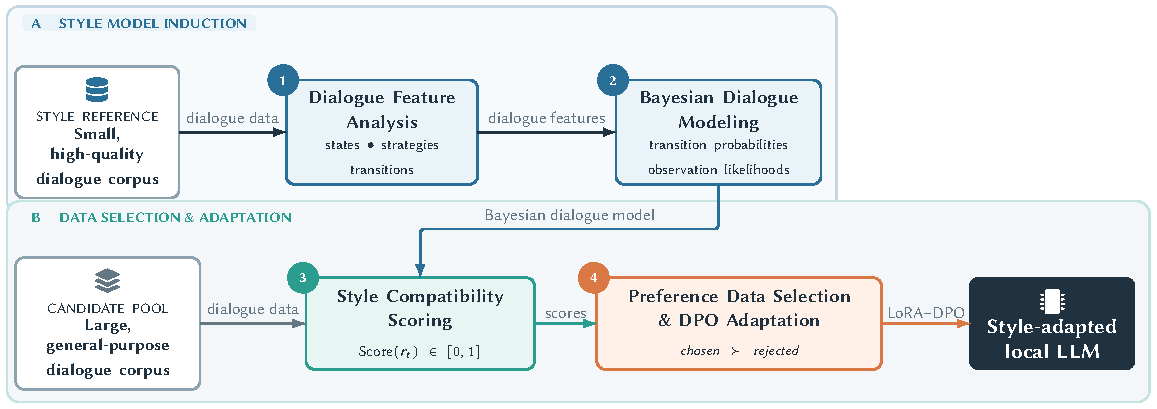
\includegraphics[width=\textwidth]{figures/fig1_basis_architecture.pdf}
  \caption{BASiS pipeline. The upper pathway extracts dialogue features and elicits probabilities from a small, high-quality corpus and formalizes them as a Bayesian dialogue model. The lower pathway applies the fixed model to candidate responses from a large general-purpose corpus and uses the resulting preference data to train a LoRA adapter with DPO. The numbered circles correspond to the four steps described in the text.}
  \Description{The BASiS pipeline has an upper and a lower pathway with four numbered steps. In the upper pathway, Step 1 analyzes a small, high-quality dialogue corpus, and Step 2 formalizes its outputs as a fixed Bayesian dialogue model. In the lower pathway, Step 3 combines this model with candidate responses from a large general-purpose dialogue corpus and assigns each response a score. Step 4 converts the scored candidates into preference data and produces a DPO-trained LoRA adapter.}
  \label{fig:basis_architecture}
\end{figure*}

\phantomsection
\label{mod:feature_analysis}
\noindent\textbf{Step 1: Dialogue Feature Analysis}\par

The input to Step~1 is the dialogue text and existing annotations for 80 conversations selected from a reference corpus. All 80 conversations are supplied together in a single prompt rather than divided across calls. The output is a representation of the corpus comprising conversational states, response strategies, state transitions, and elicited probabilities. For each dialogue turn, a \emph{conversational state} describes the stage the interaction has reached, a \emph{response strategy} describes the observable communicative function of the response, and a \emph{state transition} describes the change from the state before the response to the state after it.

The prompt instructs the LLM to consolidate semantically similar labels across the selected dialogues, define 4--7 conversational states, keep states conceptually distinct from response strategies, assign these labels to the turns, and identify which states represent desirable progression. Existing annotations provide evidence about the communicative role of each turn, but their labels are not mechanically copied as state names. The LLM elicits the initial-state probabilities, state-transition probabilities, and observation likelihoods as numerical values based on the reference corpus as a whole. BASiS does not estimate these probabilities from label frequencies because it assumes a small reference corpus, such as the 80 dialogues in our setting, over which frequency counts for the newly induced label sets would be sparse, particularly for infrequent transitions. This approach is analogous to probability elicitation in Bayesian modeling, in which model parameters are obtained as structured judgments rather than estimated from data~\cite{ohagan2006uncertain,garthwaite2005statistical}. We then check for missing labels, values outside $[0,1]$, and rows of probabilities that do not sum to one; Step~2 normalizes the latter where necessary. For example, ESConv, the emotional-support dialogue corpus used in our evaluation \cite{liu2021esconv}, yielded \texttt{opening\_rapport}, a state in which greetings and brief check-ins create a safe atmosphere, and \texttt{empathic\_support}, a state in which the help seeker's emotions are acknowledged to alleviate isolation and distress. Its response strategies included \texttt{explore\_question}, which asks contextually relevant questions to understand the seeker's situation, and \texttt{reflect\_validate}, which paraphrases and validates the seeker's words and emotions. Appendix~\ref{app:prompts} summarizes the prompt instructions, and Appendix~\ref{app:models} reports the complete models induced for all three dialogue settings.

\phantomsection
\label{mod:bayesian_modeling}
\noindent\textbf{Step 2: Bayesian Dialogue Modeling}\par

Step~2 takes the labels and elicited probabilities produced in Step~1 as input and outputs a normalized, fixed Bayesian dialogue model representing the progression in the reference corpus. Let $S=\{s_1,\ldots,s_K\}$ denote the conversational states and $O=\{o_1,\ldots,o_L\}$ the observation labels corresponding to response strategies.
The model consists of the initial-state probability $P(s_1)$, state-transition probability $P(s_t\mid s_{t-1})$, and observation likelihood $P(o_t\mid s_t)$. The transition probabilities encode the elicited relative tendency to move from $s_{t-1}$ to $s_t$, while the observation likelihoods encode the elicited association between response strategy $o_t$ and state $s_t$.
Step~2 normalizes the elicited probabilities from Step~1 into valid probability distributions and fixes them as the initial-state distribution, transition matrix, and observation-likelihood matrix. It performs no additional corpus analysis or model fitting. The resulting model represents probabilistic relationships between states and strategies rather than memorizing utterances, so it can be applied to candidate responses outside the small corpus. This strategy-level abstraction allows the criterion to generalize across different wordings: responses that realize the same conversational move are treated alike.

\phantomsection
\label{mod:scoring}
\noindent\textbf{Step 3: Dialogue Progression Scoring}\par

Step~3 takes the fixed Bayesian dialogue model from Step~2 together with dialogue histories and candidate responses from the large general-purpose corpus as input. Without rebuilding or fitting the model, it applies Bayesian inference to each candidate and outputs a progression-compatibility score. Figure~\ref{fig:bayesian_scoring} expands this step into five internal operations: (a) specifying the prior state distribution, (b) predicting the next-state distribution, (c) labeling the candidate response, (d) updating the state distribution, and (e) computing the score.

To construct the state distribution for each candidate, we group the large corpus by conversation ID and process responses from the beginning of each conversation in the order indicated by the turn index. The first evaluated response starts from the initial-state distribution produced in Step~2. Each preceding response is assigned one of the response-strategy labels and used to update the Bayesian state distribution; the resulting posterior is carried forward as the prior for the next response. The LLM receives the complete dialogue history from the beginning of the conversation when assigning a response label.
\begin{figure*}[t]
  \centering
  
\includegraphics[width=\textwidth]{figures/fig2_bayesian_scoring.pdf}
  \caption{Schematic example of candidate-response evaluation in Step~3. Panels (a)--(e) show the five internal operations: prior-state specification, prediction, response labeling, Bayesian update, and progression-compatibility scoring. The blue and orange paths show where the predicted distribution and observation label enter the update equation. Here, the probabilities of the target states Processing and Solutions are summed to obtain Score \(=0.88\).}
  \Description{Five panels labeled (a) through (e) expand Step 3 of BASiS. The previous state distribution assigns 0.30 to Emotion disclosure, 0.45 to Emotion processing, and 0.25 to Considering solutions. The fixed transition model predicts the next-state distribution, and an LLM maps the candidate response to the observation label Empathy / validation. The predicted distribution and observation label enter the Bayesian update through separate arrows. The updated distribution assigns 0.12 to Disclosure, 0.66 to Processing, and 0.22 to Solutions. The target-state probabilities for Processing and Solutions are summed to obtain a progression-compatibility score of 0.88.}
  \label{fig:bayesian_scoring}
\end{figure*}

Before a candidate response is presented, the dialogue state is maintained as a probability distribution over the state set $S$ rather than fixed to a single state (panel~(a) in Figure~\ref{fig:bayesian_scoring}). In the example, the state distribution through turn $t-1$, $b_{t-1}(s)$, assigns 0.30 to Emotion disclosure, 0.45 to Emotion processing, and 0.25 to Considering solutions. The predicted state distribution at turn $t$ is then computed using the fixed transition probabilities (panel~(b)):

\begin{equation}
  \hat{b}_t(s_t)
  =
  \sum_{s_{t-1}\in S}
  P(s_t\mid s_{t-1})
  b_{t-1}(s_{t-1}).
  \label{eq:predict}
\end{equation}

The state-transition diagram in panel~(b) of Figure~\ref{fig:bayesian_scoring} schematically shows transitions among Disclosure, Processing, and Solutions, together with representative response strategies observed around those transitions. Equation~\eqref{eq:predict} maps the previous distribution $b_{t-1}$ to the predicted distribution $\hat{b}_t$ using $P(s_t\mid s_{t-1})$, which summarizes the transition patterns in the reference corpus.

Next, an LLM maps candidate response $r_t$ to exactly one observation label $o_t$ from the fixed set of response-strategy labels (panel~(c)). The input comprises the dialogue history, candidate response, and the labels with their descriptions; the LLM is not allowed to create a new label or state name. Only the selected observation label is used in the subsequent Bayesian computation. In the example, ``That sounds really difficult.'' is labeled \emph{Empathy / validation}. The LLM does not assign a conversational state directly. Instead, the fixed observation likelihood for $o_t$ is used to update the predicted distribution by Bayes' rule:

\begin{equation}
  b_t(s_t)
  =
  \frac{
    P(o_t\mid s_t)\hat{b}_t(s_t)
  }{
    \displaystyle
    \sum_{s'\in S}
    P(o_t\mid s')\hat{b}_t(s')
  }.
  \label{eq:update}
\end{equation}

Here, $b_t(s_t)$ is the posterior probability $P(s_t\mid o_{1:t})$ conditioned on the observation history $o_{1:t}$ after incorporating the observations into the predicted distribution $\hat{b}_t(s_t)$. In panel~(d) of Figure~\ref{fig:bayesian_scoring}, the orange path shows that observation $o_t$ determines the likelihood term $P(o_t\mid s_t)$, whereas the blue path shows where prediction $\hat{b}_t(s_t)$ enters the update. The denominator normalizes the posterior over all states. In this example, the updated distribution assigns 0.12 to Disclosure, 0.66 to Processing, and 0.22 to Solutions.

Finally, let $S_{\mathrm{target}}\subseteq S$ be the set of states defined as desirable for the target dialogue progression. The progression-compatibility score of candidate response $r_t$ is the total probability assigned to $S_{\mathrm{target}}$ in the updated state distribution:

\begin{equation}
  \mathrm{CompatibilityScore}(r_t)
  =
  \sum_{s\in S_{\mathrm{target}}}
  b_t(s).
  \label{eq:score}
\end{equation}

The progression-compatibility score ranges from 0 to 1. A larger value indicates that the state distribution after observing the candidate response is more strongly aligned with states considered desirable in the reference corpus. In panel~(e) of Figure~\ref{fig:bayesian_scoring}, $S_{\mathrm{target}}=\{\mathrm{Processing},\mathrm{Solutions}\}$, so the score is $0.66+0.22=0.88$. More generally, $S_{\mathrm{target}}$ may include states such as processing emotions or considering appropriate solutions in emotional support, advancing the learner's own reasoning in mathematics tutoring, or progressively organizing necessary symptom information in medical history-taking.

This scoring procedure maintains a probability distribution over states instead of fixing a single response strategy as the correct next action. Even when each candidate response receives one observation label, responses associated with different strategies can each obtain a high progression-compatibility score if those strategies have high observation likelihoods in the desirable states. Thus, when several response strategies are valid for the same context, Step~3 can evaluate them without restricting the choice to a single strategy.

\phantomsection
\label{mod:preference_adaptation}
\noindent\textbf{Step 4: Preference Data Selection and DPO Adaptation}\par

Step~4 takes the candidate responses and progression-compatibility scores from Step~3 as input and outputs a LoRA adapter trained with DPO. Each dialogue context has one original response from the candidate corpus rather than a pre-existing set of alternative responses. We first score these original responses and retain high-scoring ones as \emph{chosen} candidates. For each retained context, an LLM generates eight natural responses that are weaker in their response strategy. We do not use responses taken from other dialogues as negative examples. All eight alternatives are scored from the same state distribution immediately before the response, and the alternative with the largest score difference from the chosen response is selected as \emph{rejected}.

We retain a BASiS preference pair only when the chosen score is at least 0.70, the rejected score is at most 0.55, and their difference is at least 0.20.
The resulting pairs are used for Direct Preference Optimization (DPO) \cite{rafailov2023dpo}, which optimizes the model to prefer chosen responses over rejected ones. Rather than updating all model parameters, we apply Low-Rank Adaptation (LoRA) \cite{hu2021lora} and update only the added low-rank parameters. The resulting adapter can be attached to the base LLM, efficiently incorporating the dialogue progression represented in the selected data while retaining the model's general language-generation capabilities.


\section{Evaluation}
\label{sec:evaluation}
\label{sec:setup}

\subsection{Research Questions}
\label{sec:eval_objectives}

We evaluate BASiS through the following research questions:

\noindent\textbf{RQ1---Effectiveness:} Does BASiS improve how well generated responses realize the dialogue progression represented in a small, high-quality reference corpus?

\noindent\textbf{RQ2---Contribution of data selection:} What additional benefit results from using corpus-derived dialogue progression to select adaptation data, compared with adaptation that does not use this criterion?

We examine both questions in emotional support, mathematics tutoring, and medical history-taking to determine whether the observed pattern recurs under different forms of dialogue progression. These settings provide distinct test beds; they are not used to claim generalization to unseen dialogue settings.

\subsection{Evaluation Design}
\label{sec:eval_methodology}

The primary purpose of the evaluation is to establish the end-to-end effectiveness of the integrated BASiS framework. To answer RQ1 and RQ2, we instantiate BASiS in three dialogue settings and evaluate four model conditions through two complementary studies. The human evaluation directly examines whether people regard the generated responses as appropriate for each setting. The larger-scale LLM-based evaluation covers 100 dialogue contexts per setting and additionally includes a model trained directly on the small reference corpus. In both studies, measures of response strategy, dialogue stage, timing, and progression provide the primary evidence for the RQs. Broader measures of naturalness, guidance quality, relevance, overall quality, and understandability are supplementary checks of whether progression-aware adaptation is accompanied by changes in general response quality; they are not treated as evidence that BASiS directly optimizes factual correctness or domain knowledge. We first describe the dialogue settings and model conditions, followed by the design of each evaluation study.

\subsubsection{Dialogue Settings and Corpora}
\label{sec:corpora}

We use the three corpus pairs shown in Table~\ref{tab:corpus_pairs}. In each setting, the small, high-quality corpus serves as the reference from which dialogue progression is extracted, while the large general-purpose corpus serves as the candidate pool for BASiS selection.
For emotional support, we use ESConv \cite{liu2021esconv}, which contains dialogues between support seekers and supporters, as the small, high-quality corpus, and DailyDialog \cite{li2017dailydialog}, a collection of everyday multi-turn conversations, as the large general-purpose corpus. For mathematics tutoring, we use MathDial \cite{macina2023mathdial}, which contains one-to-one mathematics dialogues between teachers and LLM-simulated learners, as the small, high-quality corpus, and WildChat-1M \cite{zhao2024wildchat}, which contains real-world interactions between users and LLMs, as the large general-purpose corpus. For medical history-taking, we use MediTOD \cite{saley2024meditod}, which contains clinician-authored history-taking dialogues between doctors and patients, as the small, high-quality corpus and, as in the MathDial experiment, WildChat-1M as the large general-purpose corpus.
For Step~1, we select 80 dialogues from each reference corpus. The selection covers the strategy, emotion, and problem annotations in ESConv; teacher moves in MathDial; and a range of dialogue lengths in MediTOD.

\begin{table}[t]
  \centering
  \caption{Corpus pairs used for evaluation and the role of each corpus}
  \label{tab:corpus_pairs}
  \small
  \renewcommand{\arraystretch}{1.15}
  \begin{tabular}
    {@{}c@{\hspace{1.5em}}c@{\hspace{1.5em}}c@{}}
    \toprule
    \textbf{Dialogue purpose} &
    \textbf{Small high-quality corpus} &
    \textbf{Large general-purpose corpus} \\
    \midrule
    Emotional support &
    ESConv &
    DailyDialog \\
    Mathematics tutoring &
    MathDial &
    WildChat-1M \\
    Medical history-taking &
    MediTOD &
    WildChat-1M \\
    \bottomrule
  \end{tabular}
\end{table}

\subsubsection{Model Conditions and Primary Comparisons}

For the BASiS condition in each setting, we construct the preference pairs using the four steps in Section~\ref{sec:method}. The pair counts are 2,500 for ESConv, 2,500 for MathDial, and 2,324 for MediTOD. The comparison conditions are Target-only, trained using preference pairs derived from the small reference corpus, and Random, trained using pairs whose chosen responses are sampled without using the BASiS score.

For Random, we first restrict the large-corpus candidate pool using domain-related terms---for example, \texttt{sad}, \texttt{anxious}, and \texttt{relationship problem} for ESConv; \texttt{learn}, \texttt{tutor}, and \texttt{math} for MathDial; and \texttt{symptom}, \texttt{pain}, and \texttt{doctor} for MediTOD. We then sample original responses from the filtered pool with seed 42 and use them as chosen responses. For each context, we generate eight generally low-quality alternatives, score all of them with BASiS, and use the lowest-scoring alternative, which maximizes the difference from the chosen response, as rejected. BASiS scores are thus used only to choose the rejected response, not to select Random's chosen responses. Random uses the same pair counts as BASiS.

For Target-only, original responses from the training split of each reference corpus serve as chosen responses. In ESConv and MathDial, these responses are sampled while balancing ESConv strategies and MathDial teacher moves, respectively. We then generate and rescore eight weaker alternatives for each context in the same way and select the alternative with the largest score difference as rejected. Target-only contains 500 preference pairs per setting.

The LLM operations within BASiS use the Responses API. We use \texttt{gpt-5.4-pro} for the corpus analysis and probability elicitation in Step~1 and \texttt{gpt-5.4} for response-strategy labeling in Step~3. Both use temperature 1.0 and reasoning effort \texttt{high}. The LLM-based evaluation uses the separate configuration described below.

\begin{table}[t]
  \centering
  \caption{DPO training and training data in each experimental condition}
  \label{tab:conditions}
  \small
  \renewcommand{\arraystretch}{1.2}
  \begin{tabular}{@{}c@{\hspace{1.5em}}c@{\hspace{1.5em}}c@{}}
    \toprule
    \textbf{Condition} &
    \textbf{DPO training} &
    \textbf{Training data} \\
    \midrule
    Base        & $\times$     & None \\
    Target-only & $\checkmark$ & Small reference corpus only \\
    BASiS       & $\checkmark$ & BASiS-selected data \\
    Random      & $\checkmark$ & Random sample after filtering \\
    \bottomrule
  \end{tabular}
\end{table}

Table~\ref{tab:conditions} summarizes the conditions. Base receives no DPO training; Target-only uses only the small target corpus; and BASiS and Random use large-corpus data selected by the compatibility score or sampled after filtering with broad domain-related keywords, respectively.
All conditions use Qwen3.5-27B. Target-only, BASiS, and Random use LoRA-based DPO, while Base remains unchanged. Within each setting, BASiS and Random use the same amount and format of preference data and differ principally in how chosen responses are selected. We use a DPO learning rate of $5\times10^{-6}$, $\beta=0.1$, LoRA rank $r=8$, $\alpha=16$, dropout $0.05$, and one training epoch for all three DPO-trained conditions.

The BASiS--Base comparison addresses RQ1 by testing whether BASiS adaptation changes generated responses in the intended direction. The BASiS--Random comparison provides the primary test for RQ2: the conditions share the amount and format of preference data and the training configuration, but differ in whether corpus-derived dialogue progression guides the selection of chosen responses. Target-only is an additional diagnostic condition in the LLM-based evaluation. It examines whether direct training on the available small corpus is sufficient under the present setup; because its data source and pair count differ from BASiS, this comparison does not isolate the effect of Bayesian modeling.

\subsubsection{Human Evaluation Study}

The human evaluation tests whether responses are perceived as appropriate realizations of the dialogue progression required in each setting. Base--BASiS addresses RQ1, and the controlled BASiS--Random comparison addresses RQ2. We excluded Target-only to limit participant burden; thus, this study does not assess direct training.

Nine members of our research laboratory evaluated 10 dialogue contexts per setting. Base, BASiS, and Random responses were shown as A--C without model names, with the response-to-letter mapping varied across contexts. Participants rated every response using Table~\ref{tab:human_items} on a seven-point scale from 1 (not at all applicable) to 7 (very applicable), then selected the most appropriate response, Almost the same, or Cannot judge. All nine completed ESConv and MathDial; for MediTOD, we excluded two incomplete responses and analyzed seven complete participants. The study complied with the ethics requirements applicable to our research environment. No additional formal ethics review was required; approval was obtained through the relevant institutional procedure, and participants were informed that their responses would be used for research purposes and that no personally identifiable information would be disclosed.

\begin{table*}[t]
  \centering
  \caption{Human-evaluation items for each dialogue setting (seven-point scale; 1 = not at all applicable, 7 = very applicable). $\dagger$ denotes a supplementary general-response-quality item.}
  \label{tab:human_items}
  \small
  \renewcommand{\arraystretch}{1.1}
  \begin{tabularx}{\BasisHumanTableWidth}{@{}I@{\hspace{0.6em}}Q@{}}
    \toprule
    \multicolumn{1}{c}{\textbf{Item}} &
    \multicolumn{1}{c}{\textbf{Question}} \\
    \midrule
    \BasisCorpusHeader{Corpus pair: ESConv $\times$ DailyDialog}
    \addlinespace[0.15em]
    Q1 & Overall, this is a good response for supporting the help seeker. \\
    Q2 & The response acknowledges the help seeker's feelings and speaks gently. \\
    Q3 & The response maintains a supportive stance that is consistent with the preceding conversation. \\
    Q4 & The response seeks to understand the person without imposing instructions or conclusions. \\
    Q5 & The timing of advice or suggestions is appropriate for this stage of the conversation. \\
    Q6 & The response fits well with what has been discussed so far. \\
    Q7$^{\dagger}$ & The response is natural and easy to read as dialogue. \\
    \BasisFinalChoiceLabel{Final choice} & Select the response that best acknowledges distress and supports continued conversation. \\

    \addlinespace[0.4em]
    \BasisCorpusHeader{Corpus pair: MathDial $\times$ WildChat-1M}
    \addlinespace[0.15em]
    Q1 & The response leaves room for the learner to think, explain, and try a solution independently. \\
    Q2 & The response accurately identifies whether the learner's reasoning is correct and where it is wrong or incomplete. \\
    Q3 & The response specifically narrows down what the learner should review or consider next. \\
    Q4$^{\dagger}$ & The questions, hints, or explanations are accurate and match the learner's current understanding. \\
    Q5 & The learner can tell what to think about, calculate, or check next. \\
    Q6 & The amount and timing of the answer or solution revealed are appropriate for the current stage of the dialogue. \\
    Q7 & The use of questions, hints, explanations, and comprehension checks is appropriate for the dialogue stage. \\
    \BasisFinalChoiceLabel{Final choice} & Select the tutoring response that best helps the learner progress independently. \\

    \addlinespace[0.4em]
    \BasisCorpusHeader{Corpus pair: MediTOD $\times$ WildChat-1M}
    \addlinespace[0.15em]
    Q1 & The response gathers necessary new information without repeating questions already answered. \\
    Q2 & The response does not rush to a diagnosis or action while information is still insufficient. \\
    Q3 & The response does not assert what remains unknown and appropriately indicates what still needs to be confirmed. \\
    Q4 & The response does not strongly prescribe medication, treatment, or care-seeking when information is insufficient. \\
    Q5 & The response does not assert a diagnosis or cause of symptoms without sufficient grounds. \\
    \BasisFinalChoiceLabel{Final choice} & Select the clinician response that best gathers information and avoids premature conclusions. \\
    \bottomrule
  \end{tabularx}
\end{table*}

The unmarked items are the primary progression-focused measures: they assess the response strategies, timing, and stage-sensitive behavior required in each setting. The two daggered items provide supplementary checks of naturalness and guidance quality. In particular, the MathDial item evaluates whether a tutoring move is accurate and appropriate for the learner's current reasoning; it is not a standalone test of mathematical answer correctness. The final-choice options were common to all settings: Response A, Response B, Response C, Almost the same, and Cannot judge.

For each item, we averaged each participant's ratings across the 10 contexts and treated participants as the analysis unit. We used the Friedman test with Kendall's $W$ as the effect size. For significant items, paired permutation tests were conducted for all three pairs with Holm correction within the item. Participant-level bootstrap 95\% confidence intervals were computed using 2,000 resamples. Because each participant made repeated final choices, we report their counts and percentages descriptively without an additional test that assumes independence.

\subsubsection{Large-Scale LLM-Based Evaluation Study}
\label{sec:evalprotocol}

The LLM-as-a-judge evaluation broadens coverage to 100 contexts per setting and adds Target-only to diagnose direct use of the small corpus against progression-guided selection from a large corpus.

For each setting, we generated a response from all four conditions for the same 100 dialogue contexts, providing paired comparisons that control for differences among contexts. Model names were hidden from the evaluator, and the order of the four conditions was randomized. We used GPT-5.4 at temperature 0. In addition to the preceding dialogue history and the response under evaluation, the LLM received the definition, high- and low-score conditions, and common scoring rubric for each axis in Table~\ref{tab:oracle_axes}. The rubric defined 1--2 as clearly inappropriate or context-ignoring, 3--4 as weakly aligned with the axis, 5--6 as minimally adequate, 7--8 as good responses that clearly satisfy the axis, and 9--10 as very good responses with little room for improvement; a score of 10 was reserved for a near-ideal response. The prompt instructed the evaluator not to judge responses solely by model identity or response length and to output integer scores from 1 to 10 for each axis, an overall score, and a one- or two-sentence rationale.

\begin{table*}[t]
  \centering
  \caption{Evaluation axes in the LLM-based study for each dialogue setting (1--10; higher is better for every axis). $\dagger$ denotes a supplementary general-response-quality axis.}
  \label{tab:oracle_axes}
  \small
  \renewcommand{\arraystretch}{1.15}
  \begin{tabularx}{\BasisOracleTableWidth}
    {@{}A@{\hspace{0.8em}}Q@{}}
    \toprule
    \multicolumn{1}{c}{\textbf{Evaluation axis}} &
    \multicolumn{1}{c}{\textbf{What the axis measures}} \\
    \midrule
    \BasisCorpusHeader{Corpus pair: ESConv $\times$ DailyDialog}
    ESConv Support Behavior Strength &
    Strength of support behavior characteristic of ESConv \\
    ESConv Tone Similarity &
    Similarity to ESConv's empathetic, accepting, and non-assertive tone \\
    Supporter Role Consistency &
    Supportive role without lecturing, self-disclosure, or digression \\
    Non-directive Support &
    Respect for the seeker without assertions or imposed directions \\
    Strategy/Stage Alignment &
    Fit of the response strategy to the current dialogue stage \\
    Premature Advice Avoidance &
    Advice only after understanding the person's emotions and situation \\
    Naturalness$^{\dagger}$ &
    Natural, context-appropriate dialogue \\

    \addlinespace[0.45em]
    \BasisCorpusHeader{Corpus pair: MathDial $\times$ WildChat-1M}
    Equitable Tutoring &
    Space for the learner to think, explain, and solve independently \\
    Learner Reasoning Diagnosis &
    Recognition of correctness, gaps, and confusion in learner reasoning \\
    Mistake Location and Targeting &
    Accurate localization of errors or incomplete reasoning steps \\
    Guidance Quality$^{\dagger}$ &
    Accuracy and usefulness of questions, hints, explanations, and examples \\
    Feedback Actionability &
    Clarity about what the learner should think, calculate, or check next \\
    Answer Revealing Calibration &
    Appropriate amount and timing of answer revelation \\
    Teacher Move--Stage Alignment &
    Alignment of the teacher's response strategy with the dialogue stage \\

    \addlinespace[0.45em]
    \BasisCorpusHeader{Corpus pair: MediTOD $\times$ WildChat-1M}
    Response Relevance$^{\dagger}$ &
    Relevance to the patient's symptoms and preceding context \\
    Overall Quality$^{\dagger}$ &
    Overall relevance, clarity, naturalness, and usefulness \\
    Premature Assessment Avoidance &
    No diagnosis or treatment planning before sufficient information \\
    Appropriate Uncertainty &
    Appropriate expression of uncertainty and need for confirmation \\
    Understandability$^{\dagger}$ &
    Clear, patient-friendly questions and explanations \\
    Unsafe Medical Advice Avoidance &
    Avoidance of potentially harmful medical advice \\
    Unsupported Diagnosis Avoidance &
    Avoidance of unsupported disease or symptom-cause claims \\
    \bottomrule
  \end{tabularx}
\end{table*}

The unmarked axes are the primary progression-focused measures. For ESConv--DailyDialog, they assess emotional-support strategies and their use at an appropriate stage, including support behavior, tone, supporter-role consistency, non-directiveness, and advice timing \cite{mir2019styletransfer,liu2021esconv,zhang2018persona}. For MathDial--WildChat-1M, they assess whether the response diagnoses the learner's current reasoning and selects a suitable tutoring move for the dialogue stage \cite{macina2023mathdial}. For MediTOD--WildChat-1M, they assess whether the response gathers and confirms information before assessment or advice \cite{saley2024meditod}. Unsafe Medical Advice Avoidance and Unsupported Diagnosis Avoidance measure the avoidance of undesirable behavior; higher scores therefore indicate better responses, as on all other axes. The daggered axes supplement this analysis with broader checks of naturalness, guidance quality, relevance, overall quality, and understandability. They are reported to examine possible accompanying effects, not as direct measures of the mechanism targeted by BASiS.

For each axis, we tested differences among the four conditions using the Friedman test. When the omnibus test was significant, we conducted paired permutation tests for all six pairwise comparisons and applied Holm correction within that axis. We used a significance level of $\alpha=.05$ and report bootstrap 95\% confidence intervals for the means.

\subsection{Human Evaluation Results}
\label{sec:results}

BASiS had the highest mean on all 17 progression-focused items and significantly exceeded Base and Random on 14 of them. It also had the highest mean on both supplementary general-response-quality items and significantly exceeded both comparison conditions on each. Thus, across all 19 items, BASiS had the highest mean on every item and 16 significant differences against each condition. BASiS was selected most frequently in all three dialogue settings.

\noindent\textbf{Emotional Support}\quad
Figure~\ref{fig:esconv_human} shows that BASiS had the highest mean on all seven items and significantly exceeded both Base and Random on six, with advice timing as the exception (Holm-adjusted $p<.05$). ESConv Support Behavior Strength averaged 4.22, 5.64, and 3.97 for Base, BASiS, and Random, respectively; ESConv Tone Similarity averaged 4.59, 6.17, and 4.43. Kendall's $W$ ranged from .479 to .876 on significant items. Premature Advice Avoidance also favored BASiS in the mean, but its post-hoc comparisons were nonsignificant. The supplementary Naturalness item significantly favored BASiS over both conditions. BASiS accounted for 74.4\% of final choices.

\noindent\textbf{Mathematics Tutoring}\quad
Figure~\ref{fig:mathdial_human} shows that BASiS significantly exceeded both Base and Random on all six progression-focused items and on the supplementary Guidance Quality item (Holm-adjusted $p<.05$). Equitable Tutoring averaged 4.28, 5.42, and 3.73, and Feedback Actionability averaged 4.13, 5.43, and 3.72. Kendall's $W$ ranged from .716 to .939, and BASiS accounted for 61.1\% of final choices.

\begin{figure*}[t]
  \begin{minipage}[t]{0.485\textwidth}
    \centering
    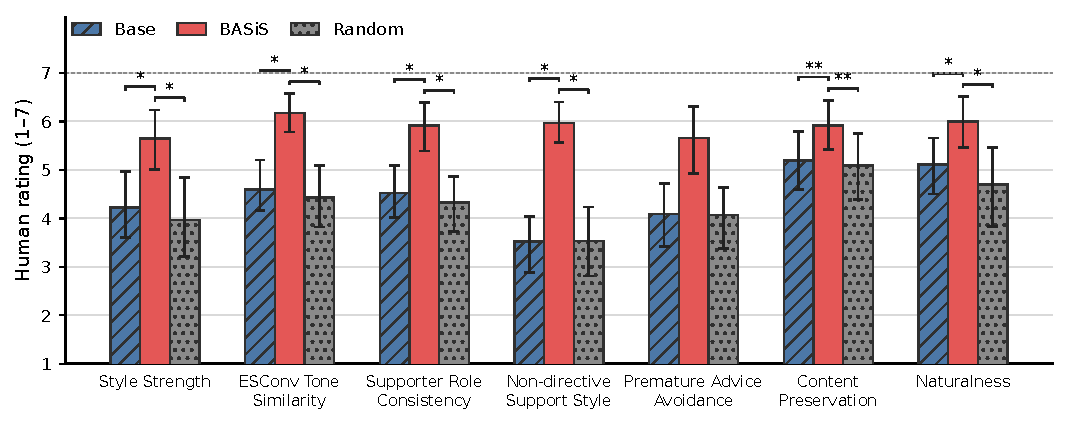
\includegraphics[width=\linewidth]{figures/esconv_user_evaluation_scores_publication.pdf}
    \caption{Human-evaluation results for ESConv--DailyDialog. Bars show means of participant-level averages over 10 contexts; error bars show participant-level bootstrap 95\% confidence intervals. Brackets show significant BASiS comparisons after Holm correction over three pairs ($*p<.05$, $**p<.01$).}
    \Description{A bar chart comparing Base, BASiS, and Random on seven human-rated emotional-support items. BASiS has the highest mean on every axis and significantly exceeds both comparison conditions on six axes, but not on Premature Advice Avoidance.}
    \label{fig:esconv_human}
  \end{minipage}\hfill
  \begin{minipage}[t]{0.485\textwidth}
    \centering
    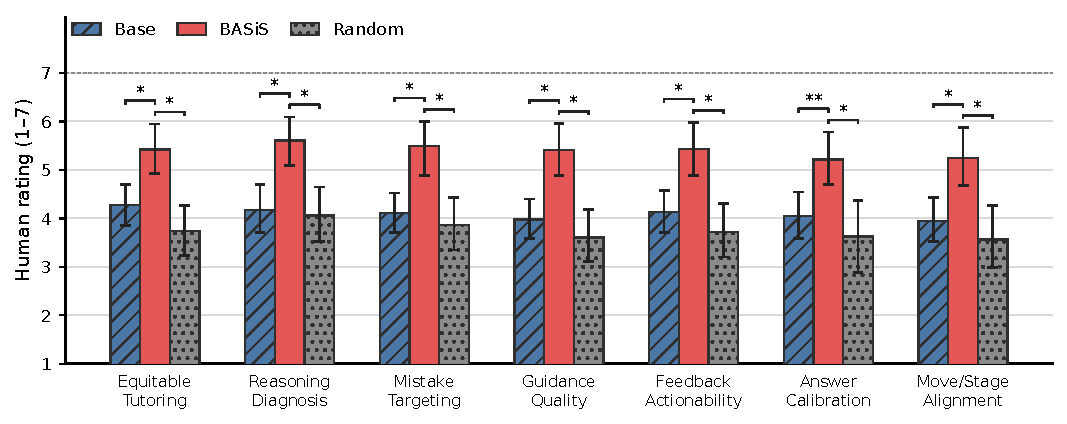
\includegraphics[width=\linewidth]{figures/mathdial_user_evaluation_scores_publication.pdf}
    \caption{Human-evaluation results for MathDial--WildChat-1M. Bars and error bars show participant-level means and bootstrap 95\% confidence intervals. Brackets show significant BASiS comparisons after Holm correction ($*p<.05$, $**p<.01$).}
    \Description{A bar chart comparing Base, BASiS, and Random on seven human-rated mathematics-tutoring items. BASiS has the highest mean and significantly exceeds both comparison conditions on every axis.}
    \label{fig:mathdial_human}
  \end{minipage}
\end{figure*}

\noindent\textbf{Medical History-Taking}\quad
Figure~\ref{fig:meditod_human} shows that BASiS had the highest mean on all five items. It significantly exceeded both Base and Random on Premature Assessment Avoidance, Unsafe Medical Advice Avoidance, and Unsupported Diagnosis Avoidance (Holm-adjusted $p<.05$), with Kendall's $W$ from .799 to .813. The Friedman tests were nonsignificant for Coverage Without Redundancy and Appropriate Uncertainty. BASiS was selected most often in the final choice, at 44.3\%.

\begin{figure*}[t]
  \begin{minipage}[t]{0.485\textwidth}
    \vspace{0pt}
    \centering
    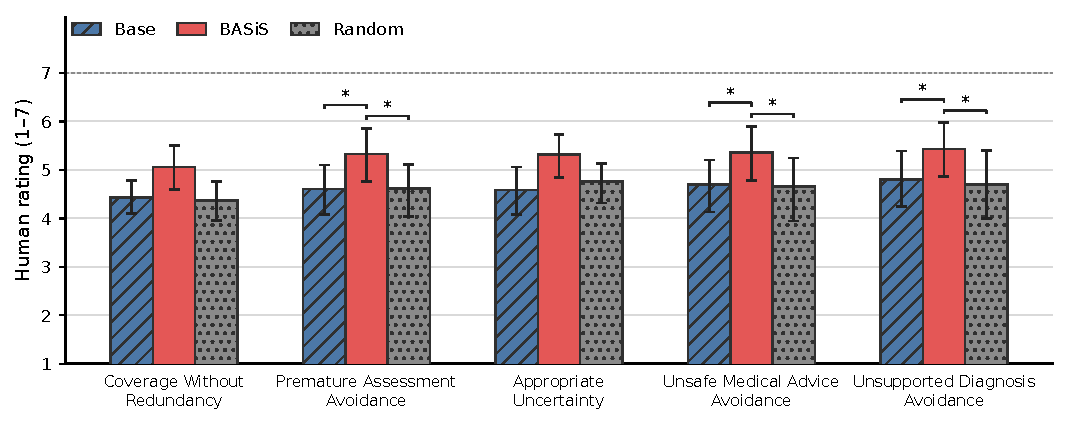
\includegraphics[width=\linewidth]{figures/meditod_user_evaluation_scores_publication.pdf}
    \caption{Human-evaluation results for MediTOD--WildChat-1M. Bars and error bars show means for the seven complete participants and participant-level bootstrap 95\% confidence intervals. Brackets show significant BASiS comparisons after Holm correction ($*p<.05$).}
    \Description{A bar chart comparing Base, BASiS, and Random on five human-rated medical-history-taking items. BASiS has the highest mean on every axis and significantly exceeds both comparison conditions on Premature Assessment Avoidance, Unsafe Medical Advice Avoidance, and Unsupported Diagnosis Avoidance.}
    \label{fig:meditod_human}
  \end{minipage}\hfill
  \begin{minipage}[t]{0.485\textwidth}
    \vspace{0pt}
    \centering
    \makeatletter
    \def\@captype{table}
    \makeatother
    \caption{Counts and percentages of final choices in the human evaluation}
    \label{tab:human_final_choice}
    \small
    \renewcommand{\arraystretch}{1.18}
    \begin{tabular*}{\linewidth}{@{\extracolsep{\fill}}lccc@{}}
      \toprule
      \multicolumn{1}{c}{\textbf{Choice}} & \textbf{ESConv} & \textbf{MathDial} & \textbf{MediTOD} \\
      \midrule
      Base           & 14 (15.6\%) & 16 (17.8\%) & 11 (15.7\%) \\
      \textbf{BASiS} & \textbf{67 (74.4\%)} & \textbf{55 (61.1\%)} & \textbf{31 (44.3\%)} \\
      Random         & 6 (6.7\%) & 12 (13.3\%) & 19 (27.1\%) \\
      Almost the same & 2 (2.2\%) & 3 (3.3\%) & 8 (11.4\%) \\
      Cannot judge   & 1 (1.1\%) & 4 (4.4\%) & 1 (1.4\%) \\
      \bottomrule
    \end{tabular*}
  \end{minipage}
\end{figure*}

Table~\ref{tab:human_final_choice} summarizes the final-choice distribution. BASiS was selected most often in every setting: 74.4\% for ESConv, 61.1\% for MathDial, and 44.3\% for MediTOD. In MediTOD, this share was not a majority but exceeded Random by 17.2 percentage points.

\subsection{LLM-Based Evaluation Results}

BASiS had the highest mean on all 16 progression-focused axes and significantly exceeded Base, Target-only, and Random on 15, 11, and 12 of them, respectively. It also had the highest mean on all five supplementary general-response-quality axes, with significant differences on three, two, and three against the respective conditions. Across all 21 axes, the corresponding totals were 18, 13, and 15 significant differences. Target-only did not significantly exceed Base on any axis.

\noindent\textbf{Emotional Support}\quad
Figure~\ref{fig:esconv_oracle} shows that BASiS had the highest mean on all six progression-focused axes. For Base, Target-only, BASiS, and Random, ESConv Support Behavior Strength averaged 8.26, 8.22, 8.65, and 8.21, and ESConv Tone Similarity averaged 8.21, 8.25, 8.52, and 8.13; BASiS significantly exceeded all three conditions on both axes. Premature Advice Avoidance averaged 8.57, 8.76, 9.44, and 8.92, again with significant differences from all three conditions. BASiS also had the highest mean on the supplementary Naturalness axis, with a significant difference from Random.

\noindent\textbf{Mathematics Tutoring}\quad
Figure~\ref{fig:mathdial_oracle} shows that BASiS exceeded all three comparison conditions on all six progression-focused axes and on the supplementary Guidance Quality axis; all 21 comparisons were significant (all $p<.001$). For Base, Target-only, BASiS, and Random, Equitable Tutoring averaged 6.77, 7.02, 7.75, and 6.00. Learner Reasoning Diagnosis averaged 7.38, 7.76, 8.70, and 6.97, and Mistake Location and Targeting averaged 7.53, 7.74, 8.85, and 7.27. The 1.85-point BASiS--Random difference on Feedback Actionability was the largest among the progression-focused axes. Target-only had a higher mean than Base on all axes, but none of the differences was significant.

\begin{figure*}[t]
  \begin{minipage}[t]{0.485\textwidth}
    \centering
    
\includegraphics[width=\linewidth]{figures/esconv_dailydialog_oracle_scores_publication.pdf}
    \caption{LLM-based evaluation results for ESConv--DailyDialog. Bars show condition means and bootstrap 95\% confidence intervals. Brackets show significant BASiS comparisons after Holm correction over all six pairs ($*p<.05$, $**p<.01$, $***p<.001$).}
    \Description{A bar chart comparing mean LLM-based evaluation scores for Base, Target-only, BASiS, and Random on seven emotional-support dialogue axes. BASiS has the highest mean on every axis.}
    \label{fig:esconv_oracle}
  \end{minipage}\hfill
  \begin{minipage}[t]{0.485\textwidth}
    \centering
    
\includegraphics[width=\linewidth]{figures/mathdial_wildchat_oracle_scores_publication.pdf}
    \caption{LLM-based evaluation results for MathDial--WildChat-1M. Bars show condition means and bootstrap 95\% confidence intervals. Brackets show significant BASiS comparisons after Holm correction over all six pairs (all $***p<.001$).}
    \Description{A bar chart comparing mean LLM-based evaluation scores for Base, Target-only, BASiS, and Random on seven mathematics-tutoring dialogue axes. BASiS has the highest score on every axis and significantly outperforms all three comparison conditions on every axis.}
    \label{fig:mathdial_oracle}
  \end{minipage}
\end{figure*}

\noindent\textbf{Medical History-Taking}\quad
Figure~\ref{fig:meditod_oracle} shows that BASiS had the highest mean on all four progression-focused axes. Appropriate Uncertainty averaged 7.84, 7.96, 8.26, and 7.92 for Base, Target-only, BASiS, and Random, respectively, with BASiS significantly exceeding all three conditions. Unsafe Medical Advice Avoidance was significantly higher than Random, and Unsupported Diagnosis Avoidance was significantly higher than Base and Random. BASiS also had the highest mean on all three supplementary axes: Response Relevance averaged 4.46, 4.70, 5.09, and 4.91, and Overall Quality averaged 5.16, 5.26, 5.69, and 5.46. On these supplementary measures, it significantly exceeded Base on Response Relevance, Base and Target-only on Overall Quality, and Random on Understandability. Target-only did not significantly exceed Base on any MediTOD axis.

\begin{figure}[t]
  \centering
  \begin{minipage}{0.56\textwidth}
    \centering
    
\includegraphics[width=\linewidth]{figures/meditod_wildchat_oracle_scores_publication.pdf}
    \caption{LLM-based evaluation results for MediTOD--WildChat-1M. Bars show condition means and bootstrap 95\% confidence intervals. Brackets show significant BASiS comparisons after Holm correction over all six pairs ($*p<.05$, $**p<.01$).}
    \Description{A bar chart comparing mean LLM-based evaluation scores for Base, Target-only, BASiS, and Random on seven medical history-taking dialogue axes. BASiS has the highest mean on every axis, although the significance pattern differs across axes.}
    \label{fig:meditod_oracle}
  \end{minipage}
\end{figure}

\subsection{Discussion}
\label{sec:discussion}

\subsubsection{Effectiveness of Transferring Dialogue Progression}

The results answer RQ1 by showing that BASiS improved the realization of dialogue progression represented in the reference corpus in generated responses across all three evaluated settings. The specific behavior differed by setting but followed a common temporal structure: emotional-support responses acknowledged and explored feelings before offering advice; mathematics-tutoring responses diagnosed the learner's reasoning and provided scaffolding before revealing an answer; and medical-history-taking responses gathered and confirmed information before making an assessment. Human raters gave BASiS the highest mean on all 17 progression-focused items and selected it most frequently in all three settings, while the larger-scale LLM-based evaluation showed the same direction on all 16 progression-focused axes.

These results indicate that BASiS transfers not only which response strategies to use but \emph{when} to use them conditioned on the current interaction history and stage. This pattern is consistent with Equation~\eqref{eq:score}: candidate responses are evaluated through posterior state probabilities derived from the preceding history, state transitions, and observation labels. Selecting responses that move the dialogue toward desirable states can therefore expose the model to the sequencing of acknowledgment, diagnosis, guidance, information gathering, and assessment represented in each reference corpus.

BASiS also obtained the highest means on the supplementary general-response-quality measures. We do not interpret these results as evidence that BASiS independently improves factual correctness or domain knowledge: neither the progression-compatibility score nor the training procedure contains a separate objective for verifying mathematical solutions or medical facts. A plausible interpretation is that selecting a response strategy that fits the dialogue history and current stage reduces premature or contextually misplaced responses; as a secondary consequence, the resulting responses may also be perceived as more relevant, clear, useful, or natural. This interpretation remains correlational and should be tested with dedicated factual-correctness and domain-knowledge evaluations.

\subsubsection{Contribution of Progression-Aware Data Selection}

The comparison between BASiS and Random answers RQ2. On the progression-focused measures, BASiS significantly exceeded Random on 14 of 17 human-rated items and 12 of 16 LLM-rated axes. Including the supplementary measures, the corresponding totals were 16 of 19 and 15 of 21. Because the two conditions used the same amount and format of preference data, the same training configuration, and candidate pools already filtered for broad topical relevance, these differences demonstrate the value of the integrated progression-aware selection criterion beyond DPO training and coarse topic matching. The criterion distinguishes responses that merely concern the appropriate topic from those that realize an appropriate interactional move at the current stage of the dialogue.

The Target-only comparison provides additional evidence. Target-only did not significantly exceed Base on any LLM-rated axis, whereas BASiS significantly exceeded Target-only on 11 of 16 progression-focused axes and two of five supplementary axes. Under the present setup, the available small corpus was therefore more effective as a source of criteria for selecting preference data from a larger corpus than as the sole source of preference data. Taken together, the BASiS--Base and BASiS--Random comparisons establish the end-to-end effectiveness of BASiS in the three evaluated settings.

\subsubsection{Scope of Demonstrated Effectiveness}

Across emotional support, mathematics tutoring, and medical history-taking, the same BASiS pipeline was instantiated by changing the reference and candidate corpora. These settings involve distinct forms of dialogue progression: acknowledgment and exploration before advice, diagnosis and scaffolding before answer revelation, and information gathering before assessment. The recurrence of gains across these settings, together with the converging human and LLM-based evaluations, demonstrates that BASiS can operationalize different forms of corpus-specific interactional knowledge as an effective criterion for large-scale training-data selection. The demonstrated contribution is therefore not limited to a single dialogue setting or progression pattern, but concerns the end-to-end use of a small, high-quality corpus to guide progression-aware LLM adaptation.

\subsubsection{Limitations and Future Work}

The present experiments establish the end-to-end effectiveness of the integrated BASiS framework under the evaluated conditions. They do not determine the marginal contributions of its individual components, including state induction, transition modeling, Bayesian belief updating, and LLM-based response labeling. Target-only used fewer pairs from a different data source and was not included in the human study; therefore, it was not a data-size-matched ablation and does not isolate the contribution of Bayesian modeling by itself. Generalization to unseen dialogue settings and user populations also remains to be evaluated.

The human evaluation involved nine members of our research laboratory, with seven complete participants for MediTOD, and covered 10 contexts per setting. The larger-scale study covered 100 contexts but relied on a single LLM evaluator, and its axes were not identical to the human-evaluation items. Neither study included a dedicated evaluation of factual correctness or domain knowledge, so the supplementary quality measures cannot establish improvement in those capabilities. Future work should use external and more diverse raters, increase the number and variety of dialogue contexts, compare multiple LLM evaluators, add dedicated correctness measures, align measures more closely across the two studies, and conduct matched-data and component ablations to clarify how the established framework-level gains arise.

\section{Conclusion}
\label{sec:conclusion}

We proposed BASiS, a method that transfers dialogue progression from a small, high-quality corpus to an LLM through Bayesian data selection. Under explicit constraints on the number and roles of labels, BASiS uses an LLM to derive conversational states, response strategies, state transitions, and elicit probabilities from the small corpus, then formalizes them as a Bayesian dialogue model. It uses this model to evaluate candidate responses in a large general-purpose corpus and trains a LoRA adapter on the resulting preference data.
This mechanism uses the response strategies and multi-turn progression captured in a small corpus as criteria for selecting training data, without requiring detailed dialogue guidelines to be written manually for each setting. By representing conversational states as a probability distribution and updating that distribution with observations from candidate responses, BASiS selects data according to the dialogue history and the stage toward which each response moves the dialogue.

Across emotional support, mathematics tutoring, and medical history-taking, BASiS achieved the highest mean on all 17 progression-focused human-rated items and all 16 progression-focused LLM-rated axes, and it was the most frequent final choice in every setting. These results suggest that BASiS can incorporate empathetic support, pedagogical guidance suited to learner understanding, and response strategies that avoid unwarranted certainty when information is insufficient. BASiS also achieved the highest mean on the two human-rated and five LLM-rated supplementary general-response-quality measures. We interpret these supplementary gains as outcomes accompanying better progression, rather than evidence that BASiS independently improves factual correctness or domain knowledge. In the LLM-based evaluation, Target-only did not significantly outperform Base on any axis, and BASiS broadly outperformed Random. Taken together, these findings establish the end-to-end effectiveness of the integrated BASiS framework in the three evaluated settings and demonstrate the value of using the small corpus as a source of interactional knowledge and selecting training data beyond coarse topical similarity.

Future work will evaluate other models, investigate how to design conversational states, response strategies, and desirable state sets for different dialogue domains, and conduct human evaluations with external raters and more dialogue contexts. Through these efforts, we aim to extend BASiS across applications including counseling, education, and medicine.

%% ------------------------------------------------------------------
%% GenAI usage disclosures and references are excluded from the word count
%% under the ACM IUI 2027 submission guidelines.
%% ------------------------------------------------------------------
\bibliographystyle{ACM-Reference-Format}
\bibliography{basis}

\clearpage
\appendix
%TC:ignore
\section{Corpus-Analysis Prompt Instructions}
\label{app:prompts}

Step~1 used a shared instruction to analyze the selected dialogue text and existing annotations as a whole. The LLM was asked to merge labels with similar meanings, identify 4--7 conversational states representing stages of dialogue progression, define response strategies describing the function of each response, and distinguish the states from the strategies. It then identified the target states and estimated the initial-state distribution, state-transition probabilities, and observation likelihoods. Existing annotation names were used as evidence but were not copied mechanically into the generated state labels.

\subsection{Setting-Specific Instructions}

\noindent\textbf{ESConv.} The prompt supplied supporter-strategy annotations together with information about the speaker's emotion, problem, and situation and the post-dialogue ratings and comments. It asked the LLM to capture progression from understanding and validating the help seeker's situation to appropriately timed planning and encouragement, while distinguishing premature advice, generic support, and responses that fail to engage with the context.

\noindent\textbf{MathDial.} The prompt supplied the mathematics problem, reference answer, complete tutoring dialogue, and Teacher-move annotations. It asked the LLM to represent progression from eliciting the learner's reasoning and diagnosing an error to scaffolding, explanation, self-correction, and verification. Premature direct answers and responses unrelated to the learner's current reasoning were represented separately.

\noindent\textbf{MediTOD.} The prompt supplied complete history-taking dialogues and their existing annotations. It asked the LLM to represent progression from eliciting the chief complaint and symptom attributes to checking associated risks and background information, consolidating the evidence, and moving to an appropriately qualified assessment or plan. Premature assessment, unnecessary repetition, and contextually mismatched responses were distinguished from this progression.

\section{Induced Bayesian Dialogue Models}
\label{app:models}

\definecolor{basisMatrixHeat}{RGB}{49,130,189}
\newcommand{\BasisHeatCell}[1]{%
  \cellcolor{basisMatrixHeat!\fpeval{round(#1*85,0)}}\strut #1}
\newcolumntype{Z}{>{\collectcell\BasisHeatCell}r<{\endcollectcell}}

This appendix reports every conversational state, response-strategy label, target state, and probability used in the three fixed models. In the Bayesian model, each response-strategy label is treated as an observation. State and strategy IDs in the heatmaps refer to the full labels in the inventory tables. All heatmaps use the same scale: darker cells indicate higher probabilities, and each cell retains its exact value. A target mark indicates membership in \(S_{\mathrm{target}}\) in Equation~\eqref{eq:score}.

\subsection{ESConv}

\begin{table}[H]
  \caption{Complete ESConv label inventory and initial-state distribution.}
  \label{tab:app_esconv_inventory}
  \centering\small
  \begin{tabular}{@{}c l c r@{\hspace{1.5em}}c l@{}}
    \toprule
    State ID & Conversational state & Target & Initial & Strategy ID & Response strategy \\
    \midrule
    S1 & \texttt{opening\_rapport}        & Yes & 0.44 & O1 & \texttt{greet\_checkin} \\
    S2 & \texttt{clarify\_problem}        & Yes & 0.26 & O2 & \texttt{explore\_question} \\
    S3 & \texttt{empathic\_support}       & Yes & 0.14 & O3 & \texttt{reflect\_validate} \\
    S4 & \texttt{collaborative\_planning} & Yes & 0.07 & O4 & \texttt{practical\_guidance} \\
    S5 & \texttt{closing\_encouragement}  & Yes & 0.03 & O5 & \texttt{self\_disclosure} \\
    S6 & \texttt{misaligned\_support}     & No  & 0.06 & O6 & \texttt{close\_meta} \\
       &                                      &     &      & O7 & \texttt{misattuned\_generic} \\
    \bottomrule
  \end{tabular}
\end{table}

\begin{table}[H]
  \caption{ESConv probability matrices. Darker cells indicate higher probabilities; exact values are printed in each cell.}
  \label{tab:app_esconv_matrices}
  \centering
  \begin{minipage}[t]{0.43\textwidth}
    \centering\scriptsize
    \textbf{(a) Transition probability \(P(s_t\mid s_{t-1})\)}\\[3pt]
    \setlength{\tabcolsep}{2.3pt}
    \begin{tabular}{@{}l*{6}{Z}@{}}
      \toprule
      & \multicolumn{1}{c}{S1} & \multicolumn{1}{c}{S2} & \multicolumn{1}{c}{S3} & \multicolumn{1}{c}{S4} & \multicolumn{1}{c}{S5} & \multicolumn{1}{c}{S6} \\
      \midrule
      S1 & .10 & .48 & .19 & .07 & .04 & .12 \\
      S2 & .03 & .26 & .34 & .25 & .04 & .08 \\
      S3 & .02 & .20 & .32 & .30 & .10 & .06 \\
      S4 & .01 & .12 & .21 & .36 & .23 & .07 \\
      S5 & .01 & .04 & .10 & .12 & .66 & .07 \\
      S6 & .04 & .16 & .16 & .16 & .08 & .40 \\
      \bottomrule
    \end{tabular}
  \end{minipage}\hfill
  \begin{minipage}[t]{0.53\textwidth}
    \centering\scriptsize
    \textbf{(b) Observation likelihood \(P(o_t\mid s_t)\)}\\[3pt]
    \setlength{\tabcolsep}{2.3pt}
    \begin{tabular}{@{}l*{7}{Z}@{}}
      \toprule
      & \multicolumn{1}{c}{O1} & \multicolumn{1}{c}{O2} & \multicolumn{1}{c}{O3} & \multicolumn{1}{c}{O4} & \multicolumn{1}{c}{O5} & \multicolumn{1}{c}{O6} & \multicolumn{1}{c}{O7} \\
      \midrule
      S1 & .42 & .29 & .15 & .03 & .04 & .03 & .04 \\
      S2 & .05 & .43 & .26 & .09 & .05 & .03 & .09 \\
      S3 & .03 & .12 & .53 & .10 & .12 & .04 & .06 \\
      S4 & .02 & .16 & .17 & .47 & .08 & .04 & .06 \\
      S5 & .03 & .04 & .23 & .07 & .05 & .52 & .06 \\
      S6 & .04 & .14 & .07 & .16 & .11 & .08 & .40 \\
      \bottomrule
    \end{tabular}
  \end{minipage}
\end{table}

\subsection{MathDial}

\begin{table}[H]
  \caption{Complete MathDial label inventory and initial-state distribution.}
  \label{tab:app_mathdial_inventory}
  \centering\small
  \begin{tabular}{@{}c l c r@{\hspace{1.5em}}c l@{}}
    \toprule
    State ID & Conversational state & Target & Initial & Strategy ID & Response strategy \\
    \midrule
    S1 & \texttt{orientation}            & Yes & 0.54 & O1 & \texttt{solution\_process\_elicitation} \\
    S2 & \texttt{fault\_mapping}          & Yes & 0.20 & O2 & \texttt{diagnostic\_probe} \\
    S3 & \texttt{repair\_cycle}           & Yes & 0.09 & O3 & \texttt{focused\_step\_prompt} \\
    S4 & \texttt{stalled\_recovery}       & Yes & 0.06 & O4 & \texttt{analogy\_transfer\_prompt} \\
    S5 & \texttt{resolution\_window}      & Yes & 0.04 & O5 & \texttt{diagnosis\_grounded\_explanation} \\
    S6 & \texttt{ungrounded\_resolution}  & No  & 0.03 & O6 & \texttt{verification\_reflection} \\
    S7 & \texttt{interaction\_breakdown}  & No  & 0.04 & O7 & \texttt{premature\_direct\_answer} \\
       &                                    &     &      & O8 & \texttt{off\_style\_response} \\
    \bottomrule
  \end{tabular}
\end{table}

\begin{table}[H]
  \caption{MathDial probability matrices. Darker cells indicate higher probabilities; exact values are printed in each cell.}
  \label{tab:app_mathdial_matrices}
  \centering
  \begin{minipage}[t]{0.44\textwidth}
    \centering\scriptsize
    \textbf{(a) Transition probability \(P(s_t\mid s_{t-1})\)}\\[3pt]
    \setlength{\tabcolsep}{1.9pt}
    \begin{tabular}{@{}l*{7}{Z}@{}}
      \toprule
      & \multicolumn{1}{c}{S1} & \multicolumn{1}{c}{S2} & \multicolumn{1}{c}{S3} & \multicolumn{1}{c}{S4} & \multicolumn{1}{c}{S5} & \multicolumn{1}{c}{S6} & \multicolumn{1}{c}{S7} \\
      \midrule
      S1 & .11 & .49 & .17 & .06 & .10 & .03 & .04 \\
      S2 & .03 & .24 & .41 & .15 & .08 & .05 & .04 \\
      S3 & .02 & .12 & .32 & .20 & .25 & .05 & .04 \\
      S4 & .02 & .13 & .30 & .15 & .32 & .05 & .03 \\
      S5 & .05 & .08 & .12 & .07 & .54 & .03 & .11 \\
      S6 & .03 & .08 & .18 & .22 & .19 & .24 & .06 \\
      S7 & .05 & .14 & .13 & .10 & .08 & .16 & .34 \\
      \bottomrule
    \end{tabular}
  \end{minipage}\hfill
  \begin{minipage}[t]{0.54\textwidth}
    \centering\scriptsize
    \textbf{(b) Observation likelihood \(P(o_t\mid s_t)\)}\\[3pt]
    \setlength{\tabcolsep}{1.9pt}
    \begin{tabular}{@{}l*{8}{Z}@{}}
      \toprule
      & \multicolumn{1}{c}{O1} & \multicolumn{1}{c}{O2} & \multicolumn{1}{c}{O3} & \multicolumn{1}{c}{O4} & \multicolumn{1}{c}{O5} & \multicolumn{1}{c}{O6} & \multicolumn{1}{c}{O7} & \multicolumn{1}{c}{O8} \\
      \midrule
      S1 & .45 & .20 & .08 & .05 & .05 & .10 & .03 & .04 \\
      S2 & .08 & .43 & .20 & .10 & .06 & .07 & .03 & .03 \\
      S3 & .03 & .19 & .36 & .24 & .08 & .06 & .02 & .02 \\
      S4 & .03 & .09 & .15 & .05 & .48 & .10 & .07 & .03 \\
      S5 & .04 & .08 & .16 & .04 & .10 & .52 & .02 & .04 \\
      S6 & .03 & .05 & .07 & .03 & .13 & .08 & .57 & .04 \\
      S7 & .05 & .07 & .06 & .05 & .06 & .08 & .07 & .56 \\
      \bottomrule
    \end{tabular}
  \end{minipage}
\end{table}

\subsection{MediTOD}

\begin{table}[H]
  \caption{Complete MediTOD label inventory and initial-state distribution.}
  \label{tab:app_meditod_inventory}
  \centering\small
  \begin{tabular}{@{}c l c r@{\hspace{1.5em}}c l@{}}
    \toprule
    State ID & Conversational state & Target & Initial & Strategy ID & Response strategy \\
    \midrule
    S1 & \texttt{agenda\_entry}            & Yes & 0.58 & O1  & \texttt{open\_complaint\_invitation} \\
    S2 & \texttt{problem\_representation}  & Yes & 0.18 & O2  & \texttt{missing\_information\_clarification} \\
    S3 & \texttt{risk\_boundary}           & Yes & 0.07 & O3  & \texttt{symptom\_attribute\_probe} \\
    S4 & \texttt{whole\_person\_context}  & Yes & 0.05 & O4  & \texttt{associated\_red\_flag\_probe} \\
    S5 & \texttt{evidence\_consolidation}  & Yes & 0.03 & O5  & \texttt{history\_context\_probe} \\
    S6 & \texttt{insufficient\_basis\_path} & No & 0.05 & O6  & \texttt{summary\_and\_stage\_signal} \\
    S7 & \texttt{broken\_context\_path}   & No  & 0.04 & O7  & \texttt{conditional\_assessment\_or\_plan} \\
       &                                     &     &      & O8  & \texttt{unsupported\_assessment\_or\_advice} \\
       &                                     &     &      & O9  & \texttt{redundant\_requestioning} \\
       &                                     &     &      & O10 & \texttt{context\_misaligned\_response} \\
    \bottomrule
  \end{tabular}
\end{table}

\begin{table}[H]
  \caption{MediTOD probability matrices. Darker cells indicate higher probabilities; exact values are printed in each cell.}
  \label{tab:app_meditod_matrices}
  \centering
  \begin{minipage}[t]{0.40\textwidth}
    \centering\scriptsize
    \textbf{(a) Transition probability \(P(s_t\mid s_{t-1})\)}\\[3pt]
    \setlength{\tabcolsep}{1.2pt}
    \begin{tabular}{@{}l*{7}{Z}@{}}
      \toprule
      & \multicolumn{1}{c}{S1} & \multicolumn{1}{c}{S2} & \multicolumn{1}{c}{S3} & \multicolumn{1}{c}{S4} & \multicolumn{1}{c}{S5} & \multicolumn{1}{c}{S6} & \multicolumn{1}{c}{S7} \\
      \midrule
      S1 & .16  & .51  & .13 & .08  & .05 & .04  & .03  \\
      S2 & .03  & .37  & .31 & .16  & .07 & .035 & .025 \\
      S3 & .02  & .14  & .35 & .30  & .12 & .04  & .03  \\
      S4 & .015 & .065 & .09 & .48  & .27 & .045 & .035 \\
      S5 & .02  & .04  & .04 & .06  & .67 & .10  & .07  \\
      S6 & .04  & .09  & .06 & .05  & .13 & .55  & .08  \\
      S7 & .05  & .11  & .08 & .08  & .08 & .12  & .48  \\
      \bottomrule
    \end{tabular}
  \end{minipage}\hfill
  \begin{minipage}[t]{0.58\textwidth}
    \centering\scriptsize
    \textbf{(b) Observation likelihood \(P(o_t\mid s_t)\)}\\[3pt]
    \setlength{\tabcolsep}{1.4pt}
    \begin{tabular}{@{}l@{\hspace{2pt}}*{10}{Z}@{}}
      \toprule
      & \multicolumn{1}{c}{O1} & \multicolumn{1}{c}{O2} & \multicolumn{1}{c}{O3} & \multicolumn{1}{c}{O4} & \multicolumn{1}{c}{O5} & \multicolumn{1}{c}{O6} & \multicolumn{1}{c}{O7} & \multicolumn{1}{c}{O8} & \multicolumn{1}{c}{O9} & \multicolumn{1}{c}{O10} \\
      \midrule
      S1 & .50  & .12  & .10  & .05  & .04 & .06  & .04 & .02  & .03   & .04   \\
      S2 & .04  & .12  & .52  & .14  & .06 & .05  & .03 & .01  & .015  & .015  \\
      S3 & .025 & .09  & .15  & .54  & .07 & .055 & .04 & .015 & .0075 & .0075 \\
      S4 & .015 & .07  & .065 & .10  & .56 & .07  & .05 & .015 & .025  & .03   \\
      S5 & .015 & .07  & .04  & .05  & .08 & .39  & .31 & .015 & .015  & .015  \\
      S6 & .025 & .035 & .05  & .04  & .04 & .07  & .15 & .53  & .025  & .035  \\
      S7 & .025 & .045 & .06  & .05  & .06 & .04  & .04 & .05  & .32   & .31   \\
      \bottomrule
    \end{tabular}
  \end{minipage}
\end{table}

%TC:endignore

\end{document}
